\documentclass[
a4paper,
pagesize,
pdftex,
12pt,
twoside, % + BCOR darunter: für doppelseitigen Druck aktivieren, sonst beide deaktivieren
BCOR=5mm, % Dicke der Bindung berücksichtigen (Copyshop fragen, wie viel das ist)
ngerman,
fleqn,
final,
]{scrartcl}
\usepackage{ucs}
\usepackage[utf8x]{inputenc} % Eingabekodierung: UTF-8
\usepackage{fixltx2e} % Schickere Ausgabe
\usepackage[T1]{fontenc} % ordentliche Trennung
\usepackage{lmodern} % ordentliche Schriften
\usepackage[unicode=true]{hyperref}
\usepackage{setspace,graphicx,tikz,tabularx} % für Elemente der Titelseite
\usepackage[draft=false,babel,tracking=true,kerning=true,spacing=true]{microtype} % optischer Randausgleich etc.

\usepackage[margin=1in]{geometry}
\usepackage{graphicx}
\usepackage{amsthm, amsmath, amssymb}
\usepackage{setspace}\onehalfspacing
\usepackage[loose,nice]{units} %replace "nice" by "ugly" for units in upright fractions
\usepackage{color}
%\usepackage{hyperref}


\usepackage{xcolor}
\definecolor{ltgrey}{HTML}{F5F5F5}

\hypersetup{
	colorlinks=true,
	linkcolor=blue,
	filecolor=magenta,      
	urlcolor=cyan,
	citecolor=blue
}

\usepackage[inline]{enumitem}
\usepackage{todonotes}

\usepackage{refcheck} %show which refs are note used
\usepackage{breakcites}

\usepackage{minted}
\usepackage{listings}

%\urlstyle{same}

\usepackage{pbox}
\usepackage{csquotes}




% Use “\cite{NEEDED}” to get Wikipedia-style “citation needed” in document
%\usepackage{ifthen}
%\let\oldcite=\cite
%\renewcommand{\cite}[2]{\ifthenelse{\equal{#2}{NEEDED}}{\textcolor{red}{\ensuremath{^\texttt{[citation~needed]}}}}{\oldcite{#1}{#2}}}

\newcommand{\citationneeded}{\textsuperscript{\color{red} [citation needed]}}
\newcommand{\toDo}[1]{\textcolor{red}{TODO: {#1}}}
 
 
% \title{E-learning performance optimization. Towards an emotionally-aware visual interface}
% Viability of an emotionally-aware interface within e-learning to optimize performance
% \author{Oleg Bystrov, Humboldt Universitaet zu Berlin}
% \date{2018}
 
\begin{document}

% LaTeX-Vorlage für die Titelseite und Selbständigkeitserklärung einer Abschlussarbeit
% basierend auf der vorigen Institutsvorlage des Instituts für Informatik
% sowie der Vorlage für Promotionsarbeiten.
%
% erweitert: 2014-06-12 Dennis Schneider <dschneid@informatik.hu-berlin.de>

% gepunktete Linie unter Objekt:
\newcommand{\TitelPunkte}[1]{%
  \tikz[baseline=(todotted.base)]{
    \node[inner sep=1pt,outer sep=0pt] (todotted) {#1};
    \draw[dotted] (todotted.south west) -- (todotted.south east);
  }%
}%

% gepunktete Linie mit gegebener Länge:
\newcommand{\TitelPunktLinie}[1]{\TitelPunkte{\makebox[#1][l]{}}}

\makeatletter

\newcommand*{\@titelTitel}{Titel der Arbeit}
\newcommand{\titel}[1]{\renewcommand*{\@titelTitel}{#1}} % Titel der Arbeit
\newcommand*{\@titelArbeit}{Arbeitstyp}
\newcommand{\typ}[1]{\renewcommand*{\@titelArbeit}{#1}} % Typ der Arbeit
\newcommand*{\@titelGrad}{akademischer Grad}
\newcommand{\grad}[1]{\renewcommand*{\@titelGrad}{#1}} % Akademischer Grad
\newcommand*{\@titelAutor}{Autor}
\newcommand{\autor}[1]{\renewcommand*{\@titelAutor}{#1}} % Autor der Arbeit
\newcommand*{\@titelGeburtsdatum}{\TitelPunktLinie{2cm}}
\newcommand{\gebdatum}[1]{\renewcommand*{\@titelGeburtsdatum}{#1}} % Geburtsdatum des Autors
\newcommand*{\@titelGeburtsort}{\TitelPunktLinie{5cm}}
\newcommand{\gebort}[1]{\renewcommand*{\@titelGeburtsort}{#1}} % Geburtsort des Autors
\newcommand*{\@titelGutachterA}{\TitelPunktLinie{5cm}}
\newcommand*{\@titelGutachterB}{\TitelPunktLinie{5cm}}
\newcommand{\gutachter}[2]{\renewcommand*{\@titelGutachterA}{#1}\renewcommand*{\@titelGutachterB}{#2}} % Erst- und Zweitgutachter
\newcommand*{\@titelEinreichungsdatum}{\TitelPunktLinie{3cm}} % Datum der Einreichung, wird nicht vom Studenten ausgefüllt
\newcommand*{\@titelVerteidigungsdatum}{} % Verteidigungstext, wird nicht vom Studenten ausgefüllt
\newcommand{\mitverteidigung}{\renewcommand*{\@titelVerteidigungsdatum}{defended on: \,\,\TitelPunktLinie{3cm}}} % Verteidigungsplatzhalter erzeugen
\newcommand*{\@wastwoside}{}

% Titelseite erzeugen:
\newcommand{\makeTitel}{%
	% Speichere, ob doppelseitiges Layout gewählt wurde:
\if@twoside%
	\renewcommand*{\@wastwoside}{twoside}
\else
	\renewcommand*{\@wastwoside}{twoside=false}
\fi
	\KOMAoptions{twoside = false}% Erzwinge einseitiges Layout (erzeugt eine Warnung)

	\begin{titlepage}
		% Ändern der Einrückungen
		\newlength{\parindentbak} \setlength{\parindentbak}{\parindent}
		\newlength{\parskipbak} \setlength{\parskipbak}{\parskip}
		\setlength{\parindent}{0pt}
		\setlength{\parskip}{\baselineskip}

		\thispagestyle{empty}

		\begin{minipage}[c][3cm][c]{12cm}
			\textsc{%
				% optischer Randausgleich per Hand:
				\hspace{-0.4mm}\textls*[68]{\Large Humboldt-Universität zu Berlin}\\
				\normalsize \textls*[45]{
					Mathematisch-Naturwissenschaftliche Fakultät\\
					Institut für Informatik
				}
			}
		\end{minipage}
		\hfill


		% Also wenn schon serifenlose Schriften (Titel), dann ganz oder gar nicht
		\sffamily

		\vfill

		\begin{center}
		\begin{doublespace}
			\vspace{\baselineskip}
			{\LARGE \textbf{\@titelTitel}}\\
			%\vspace{1\baselineskip}
			{\Large
				\@titelArbeit\\
				in fulfillment of the requirements for the degree of\\
				\@titelGrad
				\vspace{\baselineskip}
			}
		\end{doublespace}
		\end{center}

		\vfill
\newcolumntype{L}{>{\raggedright\arraybackslash}X}
		{\large \raggedleft
			\begin{tabularx}{\textwidth}{l@{\,\,\raggedright~}L} % verbreiterter Abstand zwischen Feldern wurde gewünscht
				submitted by: & \@titelAutor\\
				born on: & {\@titelGeburtsdatum}\\
				born in: & \@titelGeburtsort
				\vspace{0.5\baselineskip}\\
				submitted to: & \@titelGutachterA \\
					& \@titelGutachterB
				\vspace{0.5\baselineskip}\\
				submitted on: & \@titelEinreichungsdatum \hfill \@titelVerteidigungsdatum
			\end{tabularx}}
			\vspace{-1\baselineskip}\\\phantom{x} % Übler Hack, um eine Warnung wg. einer zu leeren hbox zu verhindern
		% Wiederherstellen der Einrückung
		\setlength{\parindent}{\parindentbak}
		\setlength{\parskip}{\parskipbak}
	\end{titlepage}

	% Aufräumen:
	\let\@titelTitel\undefined
	\let\titel\undefined
	\let\@titelArbeit\undefined
	\let\typ\undefined
	\let\@titelGrad\undefined
	\let\grad\undefined
	\let\@titelAutor\undefined
	\let\autor\undefined
	\let\@titelGeburtsdatum\undefined
	\let\gebdatum\undefined
	\let\@titelGeburtsort\undefined
	\let\gebort\undefined
	\let\@titelGutachterA\undefined
	\let\@titelGutachterB\undefined
	\let\gutachter\undefined
	\let\@titelEinreichungsdatum\undefined
	\let\einreichungsdatum\undefined
	\let\@titelVerteidigungsdatum\undefined
	\let\verteidigungsdatum\undefined

	\KOMAoptions{\@wastwoside}% Stelle alten Modus (ein-/doppelseitig) wieder her
	\let\@wastwoside\undefined
	\cleardoublepage % ganzes Blatt für die Titelseite
}

% Als Allerallerletztes kommt Selbständigkeitserklärung:
% Aufruf mit dem Datum in deutscher und englischer Form
\newcommand{\selbstaendigkeitserklaerung}[1]{%
	\cleardoublepage% Wieder auf eine eigene Doppelseite
	{\parindent0cm
		\subsection*{Selbständigkeitserklärung}
		Ich erkläre hiermit, dass ich die vorliegende Arbeit selbständig verfasst
		und noch nicht für andere Prüfungen eingereicht habe.
		Sämtliche Quellen einschließlich Internetquellen, die unverändert oder
		abgewandelt wiedergegeben werden, insbesondere Quellen für Texte, Grafiken,
		Tabellen und Bilder, sind als solche kenntlich gemacht. Mir ist bekannt,
		dass bei Verstößen gegen diese Grundsätze ein Verfahren wegen
		Täuschungsversuchs bzw. Täuschung eingeleitet wird.
		\vspace{3\baselineskip}

		{\raggedright Berlin, den #1 \hfill \TitelPunktLinie{8cm}\\}
%		\vspace{3\baselineskip}
%
% 		\selectlanguage{english}
% 		\subsection*{Statement of authorship}
% 		Hier würde die englische Selbständigkeitserklärung folgen, falls gewünscht. Doch es fehlt eine akzeptable Übersetzung.
% 		\vspace{3\baselineskip}
%
% 		Berlin, #2 \hfill \TitelPunktLinie{6cm}
	}
}%

\makeatother

	
\titel{E-learning performance optimization - towards an emotionally-aware visual interface} % Titel der Arbeit
\typ{Master Thesis} % Typ der Arbeit:  Diplomarbeit, Masterarbeit, Bachelorarbeit
\grad{Master of Science (M. Sc.)} % erreichter Akademischer Grad
% z.B.: Master of Science (M. Sc.), Master of Education (M. Ed.), Bachelor of Science (B. Sc.), Bachelor of Arts (B. A.), Diplominformatikerin
\autor{Oleg Bystrov} % Autor der Arbeit, mit Vor- und Nachname
\gebdatum{1.5.1991} % Geburtsdatum des Autors
\gebort{Potsdam, Germany} % Geburtsort des Autors
\gutachter{Prof. Dr. Niels Pinkwart}{Prof. Dr. Albrecht Schmidt} % Erst- und Zweitgutachter der Arbeit
\mitverteidigung % entfernen, falls keine Verteidigung erfolgt
\makeTitel

% -----------------------------
% --- frontmatter: Contents ---
% -----------------------------
\tableofcontents

% -------------------------------
% --- main body of the thesis ---
% -------------------------------
\clearpage

\section{Introduction}

[TODO: Intention, hypotheses and results of the study]

\clearpage

\section{Background}

	\subsection{Motivation}
	
	[TODO]
	
	E-learning providers are looking to improve the learning experience of their users and make progress as effective as possible. 
During a typical learning session each learner is subject to a range of volatile emotional states that help or hinder their learning success. 
Several factors and stimuli, both internal and external, can influence emotions. 
When we take this knowledge about emotions into account a new way to manage a learning session opens. We can incorporate this knowledge into learning sessions and provide a more appropriate task and interface for the learner.

The goal of the paper is to examine a relationship between the emotional aspect of a user interface in an e-learning system and its effect on the performance of the learner.


\begin{center}
	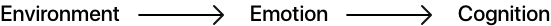
\includegraphics[width=200px]{graphics/relation1.png}
\end{center}
 
There is strong evidence of the surrounding environment having an influence on emotion \cite{Johnson2000, Arockiam2013, Bertamini2013}. This includes, for example, an e-learning system on the screen in front of the learner. In a similar fashion several studies have shown a correlation between emotion and cognition (Section \ref{sec:emotion-cognition}).

\begin{center}
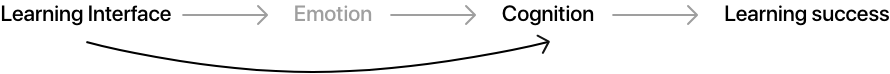
\includegraphics[width=300px]{graphics/relation2.png}
\end{center}

There is a logical argument of the existence of a transitive relation between these parameters, which could confirm the dependency of the edge variables. 
I.e. exposure to several interfaces each with a different emotional charge during an on-line lesson should lead to a difference in performance when working on the same task.
Insufficient research confirming this connection and explaining the effects has been published yet. 

In this paper I would like to explore to which extent the final parameter "learning success" can be influenced with the limited surface of contact that can be addressed through a learning interface on the screen.
	
		
	\subsection{Research basis} 
	
	\cite{McCrudden2017} describe from a standpoint of information architecture the effect of different types of visual display on cognitive processing. They highlight the important aspects of visual guidelines, the basics of human working and long-term memory and a way to quantify those under processing efficiency.
	
	There is, however, a case to be made with respect to the same visual display presented to a participant under differentiating emotional conditions. There is strong evidence that emotions play a role in information processing and, as a consequence have an effect on the resulting performance
	
	\subsection{Hypotheses}
	
	\paragraph{Hypothesis 1.} Two different interfaces can result in a significant difference in emotional response
	\paragraph{Hypothesis 2.} Resulting performance (as measured by selected study design parameters) during the experiment is higher for saturated interface, compared to desaturated interface.

\section{Approach and Methods}

To facilitate the study I make assumptions about the medium in which e-learning is usually conducted. Based on the research basis I define study design parameters and a set of target variables that will be evaluated.

	\subsection{Medium}
	
	The study is to be conducted online under a "real-life" scenario. This means, that the experiment is to be run in a browser-capable web-application runnable on modern personal computers. Like most e-learning software the  application used in the study is browser-based and usually used in users homes or public places.
	
	\subsection{Study design}
	
	The goal of the current study is to determine emotional response to provided emotional design implementation (Interface 1) compared to the control group that was provided with a stricter desaturated design (Interface 0). The differences include use of color, shapes, language, font style, responsiveness, animation. The similarities and, thus constant variables, across both interfaces include any accessibility features and general usability heuristics, such as contrast ratio level, size and placement of elements on a screen, 
	
	\begin{enumerate}
		
		\item[0.] \textbf{Clustering:} Each participant is assigned an interface version (1 of 2) and the preconditioning group (1 of 4) at random before first load of the application.
		
		\item \textbf{Preconditioning:} Each participant is shown a set of emotional images and preconditioned to be in one of 4 states:
			\textbf{1}: Positive valence / high arousal;
			\textbf{2}: Negative valence / high arousal;
			\textbf{3}: Positive valence / low arousal;
			\textbf{4}: Negative valence / low arousal;
			
		Choice and showing of preconditioning is described further in in the following chapter \ref{preconditioning}
			
		\item \textbf{Emotional validation:} A short emotional self-reporting questionnaire (SAM \ref{'sec:selfeval'}) is used to validate, whether preconditioning has had sufficient and expected effect on the participant.
		
		\item \textbf{Experiment 1:} Slightly modified classic memory game. The participant is presented with a grid of tiles, each tile containing an image. During 5 seconds at the beginning of the experiment all tiles are open to allow to memorize the images. After which all images are hidden. Only 2 tiles can be opened at any one time. Once 2 of the same tiles are open they are marked as solved. The goal is to solve all tiles.
		
		\item \textbf{Experiment 2:} Remote Associates Test (RAT). A generalized creativity test developed by Mednick \cite{Mednick1962} in 1962. Each participant is presented with a number of word sets. Each set consists of 3 words that are shown to the participant and one target word that is hidden from the them. The target word is semantically connected to all 3 visible words
		
		\item \textbf{Emotional validation:} A second emotional self-reporting questionnaire (SAM \ref{'sec:selfeval'}) to establish, whether and which effect tasks and interface have had on the participant's emotion.
		
		\item \textbf{Demographic data:} Final step adds additional context data about the person for each participant through a questionnaire to complement data analysis.
		
		
	\end{enumerate}
	
	\subsection{Preconditioning sequences} \label{preconditioning}
	
	\paragraph{Finding a preconditioning sequence}
To facilitate emotional conditioning I selected a specialized sequence containing images with a corresponding emotional charge.
Each sequence contains 21 to 39 \todo{more precise} images with each displayed for about 5 seconds.

Each subject is assigned one of four preconditioning sequences. Each sequence is aimed to condition the subject into one of the 4 quadrants, described though a valence-arousal emotional model. To simplify we will label (\ref{fig:valence_arousal_model}) them as:
\begin{enumerate}
	\item Angry (Quadrant 1)
	\item Happy (Quadrant 2)
	\item Sad (Quadrant 3)
	\item Relaxed (Quadrant 4)
\end{enumerate}


\begin{figure}
\begin{center}
	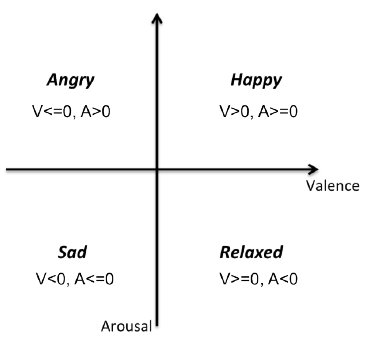
\includegraphics[width=150px]{graphics/Valence-Arousal-model-showing-the-quadrants-of-the-four-emotion-tags-used-in-this_W640.jpg}
	\caption{Valence Arousal Model \cite{Song2013} \label{fig:valence_arousal_model}}
	
\end{center}
\end{figure}

There are several emotional image data-sets available for academic purposes such as GAPED \cite{Dan-Glauser2011}, OASIS \cite{Kurdi2017}, IAPS \cite{Lang1997} and NAPS \cite{Marchewka2014}. While NAPS is offering the highest realism and quality of images, the range images seems to cover "sad" and "happy" to a less pronounced degree. In general, strong negative valence values are accompanied with high arousal values across all analyzed data-sets. Causing sadness is a challenging task. In current preconditioning sequences I am using the \textbf{OASIS} database. It has relatively wide spread of emotions compared to other sets.

Keeping in mind the need for a clear separation between groups in terms of their emotional state into account, I limited emotional images to moderately strong stimuli values, thus avoiding extreme reactions and unrealistic emotional states. It can be assumed that in most cases, people who attend e-learning lessons will have moderate levels of emotional charge. It is important to note that quadrant 1 - angry and quadrant 2 - happy has a more pronounced representation in emotional databases due to an easier and more prevalent stimuli availability. As such quadrant 1 and quadrant 2 have stronger stimuli compared to quadrant 3 and 4. It is expected that there will be a significant difference between emotion ratings of participants across these groups.

It is understood that the e-learning interface under real conditions will only cause mild-to-moderate changes to a mood.


\begin{figure}
	\centering
	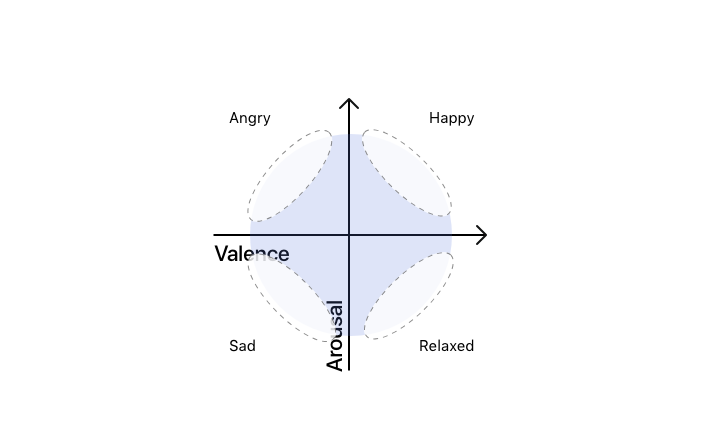
\includegraphics[width=0.7\linewidth]{graphics/Valence-Arousal-Model-1.png}
	\caption{Focus levels of emotional states on valence arousal model}
	\label{fig:valence-arousal-model-2}
\end{figure}

Illustration \ref{fig:valence-arousal-model-2} highlights with dashed outline areas the target arousal and valence values

	
	\subsection{Emotional Design Features}
	
	[TODO:] white about emotional design, rewrite citation blocks below
	
	% \clearpage

\paragraph{Developing a high performing interface}

There is a multitude of studies that analyze user interface design and user emotion. In following I will summarize them in respect to UI features tailored towards high performance

\paragraph{Literature review}

A paper by L. Arockiam et al \cite{Arockiam2013} describes that, based on previous research and their own findings optimal ui can be achieved based on a person's personality traits. We will limit ourselves to a universal set of changes that should evoke high arousal, positive valence and therefore have an effect on learning outcome, rather than look for their preference. Nevertheless it is worth mentioning...

Color - PHYSIOLOGICAL

Wilson (1966) reported higher GSR measurements for red as opposed to green, and Nourse and Welsh (1971) reported higher GSR readings for violet than green. Using 24 male college students as subjects and saturated samples of red, yellow, green, and blue as stimulus materials, Jacobs and Hustmyer (1974) found that red was significantly more arousing than either yellow or blue, and green more than blue. Using 40 undergraduate students as subjects, Jacobs and Suess (1975) found that red and yellow resulted in higher anxiety state scores than blue or green when measured by the StateTrait Anxiety Inventory. Bloomer (1976) also reported that red increases heart rate. There appears to be some evidence that spectral extremes, especially red, cause greater arousal than mid-spectral colors. This may relate to the fact that wavelengths at the extremes of the spectrum, such as red and violet, focus at different points in the eye than wavelengths at the middle of the spectrum. \cite{Pert1996}

Color - PSYCHOLOGICAL

The selected order of preference was: (1) blue, (2) red, (3) green, (4) violet, (5) orange, (6) yellow. This selection agreed with the average rankings of color preference among 21,060 subjects reported in earlier investigations. The order was the same for all races and for men and women with one exception. Men chose orange over yellow whereas women chose yellow over orange. \cite{Pert1996}

no significant differ- ences between men and women or between subjects of different races.\cite{Pert1996}

girls of all ages preferred higher value, brighter, colors as compared to boys (Child, et al., 1968) \cite{Pert1996} (study among school age children from 1 to 12 grade)

Results on the evaluation scale supported the general preference for cool colors(bl~e and green) as compared with warm colors(red and yellow) and agree with previous findings by Adams and Osgood (1973) that red is a potent color while gray and black have low potency. \cite{Pert1996}

In a color-effectiveness study conducted at Fort Monmouth, typical army training procedures were used with 11 different television lessons (Kanner and Rosenstein, 1960). No significant
differences were found in learning between
monochrome and colored versions \cite{Pert1996}

Schaie (1966) pointed out that color prefer-
ences vary from individual to individual and relate to personality. \cite{Pert1996}

(so far black and white and color has not yielded any significant difference in learning) but "colored mate- rials are preferred by learners." \cite{Pert1996}

1972: those who viewed colored transparencies had had a more positive attitude toward transparencies than \cite{Pert1996}

In a research study on color coding, Lamberski and Dwyer (1983) concluded that color is an attention-getting device that can provide measurable effects on learning that cannot be accounted for by words and labels. \cite{Pert1996}

Search Tasks: 
gain in efficiency, indicated by decreased search time, with codes of up to five colors \cite{Pert1996}

Color was found to be useful in grouping information

color versions resulted in higher recognition- memory scores (immediate recognition memory test)\cite{Pert1996}

as the variable of visual complexity increases, so does the degree of recall. (Berry (1991a)) \cite{Pert1996}

The key factor relating to color and cogni-
tive learning seems to be that it is of value when it emphasizes relevant cues, is used as a coding device, or when it is a part of the con- tent to be learned (Dwyer and Lamberski, 1982- 83; Levie, 1973; Pruisner, 1993; Wedell \& Alden, 1973). \cite{Pert1996}

Non-objective Measures

(Scanlon, 1970). Scanlon suggests that the color versions (Grey Cup football game) create emotional effects that detract from attention to details.







Colors at the ends of the spectrum, red and
violet, seem to result in greater arousal, and
colors in the middle of the spectrum, yellow,
green, cyan, seem to be best for discriminating
detail. \cite{Pert1996}
	
	\subsection{Experiments}

		\subsubsection{Experiment 1: Short term Memory}
		
		Memory Experiment 
		
		[TODO:] Describe basis of the experiment
		
		[TODO:] describe activity logging for EXP1 here?
		
		[TODO:] measuring performance of this experiment
		
		\paragraph{Performance parameters:} \label{sec:memory-parameters}
		
		\subsubsection{Experiment 2: Creative thought}
		
		A generalized creativity test developed by Mednick \cite{Mednick1962} in 1962. It does not require prior knowledge of any particular subject. Some of 144 compound remote associate sets are taken from \cite{Bowden}. These are a subset of RAT problems and have been alternatively described as "compound word problems". Of the triad of words that are presented each can form a compound word or a two-word phrase with the solution word.
		
		[TODO:] describe activity logging for EXP2 here?
		
		[TODO:] measuring performance of this experiment


	\subsection{Means of emotional self-evaluation} \label{'sec:selfeval'}
	
	

% \todo[inline, size=\tiny]{'Valence and Arousal evaluation techniques'}




	\subsection{E-learning activity logging}
	
	To assess performance of subjects several measurements are taken during the test, these differentiate between the 2 experiments.
	
	Describe general approach to recording actions and recording approach for this study.
		
		\paragraph{Current implementation} -
		
		[TODO:] describe how I implemented tracking, storage and analysis for current study
		
		\paragraph{xAPI adaptation} - 
		
		[TODO:] explore adaptability and possible constraints

\section{Study implementation}

\paragraph{Participant sourcing} 
This study includes participants attained through multiple sources:
\begin{itemize}
	\item{Local university:} On-site supervised experiments were conducted on a limited scale to facilitate a clean sample of participants and uncover problems during the study
	
	\item{Local workplace:} On-site semi-supervised experiments are conducted on a limited scale in Berlin area in Germany to facilitate a more diverse sample while keeping controlled environment conditions, similar to university experiments.
	
	\item{Social media:} Remote participants are invited to participate in unsupervised experiments on their own. Channels such as social media, interest groups and university mailing lists are used.
	
	\item{Mechanical turk:} MTurk is one of popuar web services to source participants. Previous research has shown that it can be considered a reliable platform for conducting objective studies. MTurk participants receive monetary compensation for participation \cite{Buhrmester2011a}. Mturk participants are excluded from motivation with a chance on winning a voucher prize (they do not see the field and information box about it), instead regular participant reward through MTurk is used.
	
\end{itemize}

Local and social media experiments provided additional motivation of participation with the promise of a chance to win a 20 Euro Amazon-voucher.

\section{Results and Evaluation}

[TODO:] Here describe how evaluation was done, how many people participated, demographics data.

[TODO:] Show general statistical data

	\subsection{Hypothesis 1}: 
	
	[Note:] H1 should be checked in the context of the whole app
	
	\subsection{Hypothesis 2}: 
	
	[Note:] H2 should be checked for each task separately

\section{Further research and implications of the study}

\subsection{Ethical, legal and social implications}

[TODO]

\section{Notes}






\clearpage

% ----------------
% --- appendix ---
% ----------------

\appendix

% figures
%\newpage
%\section{Figures}

\begin{figure}[h!]
	\centering
	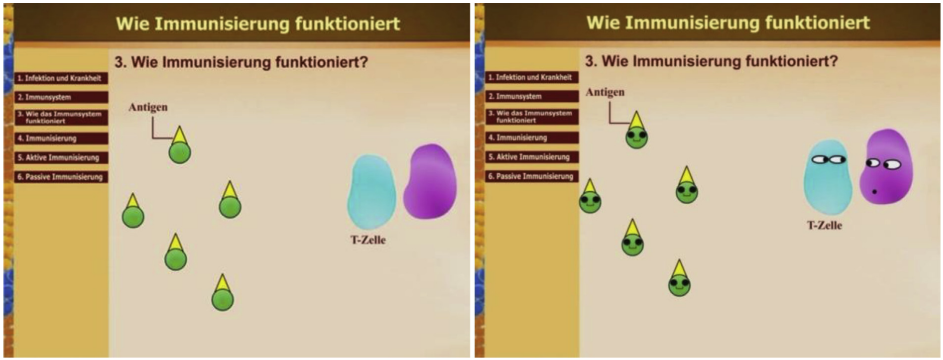
\includegraphics[width=1\linewidth]{graphics/anthropomorphisms}
	\caption{Screenshots of the learning program in the neutral version (left) and the positive version with anthropomorphisms (right). Taken from \cite{Park2015}}
	\label{fig:anthropomorphisms}
\end{figure}

\begin{figure}
	\centering
	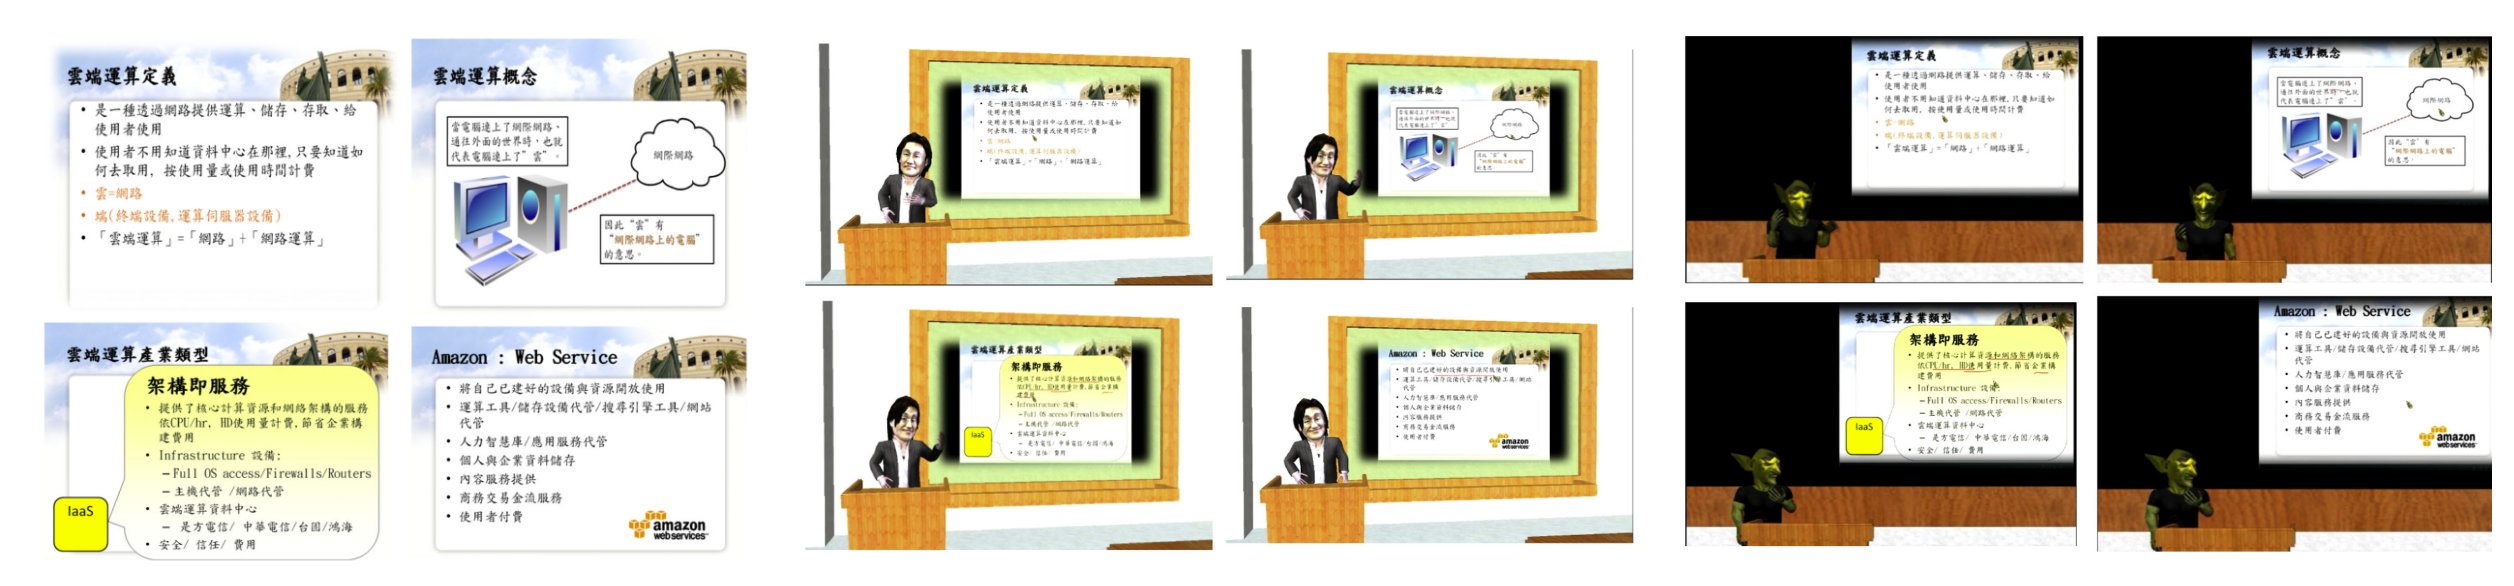
\includegraphics[width=1\linewidth]{graphics/The_effects_of_multimedia_instructional_materials}
	\caption{The effects of various multimedia instructional materials. Left to right - control group interface, experimental Group I interface (human-like animated character) and experimental Group II interface (monster-like animated character). From \cite{Lee2014}}
	\label{fig:theeffectsofmultimediainstructionalmaterials}
\end{figure}

\begin{figure}
	\centering
	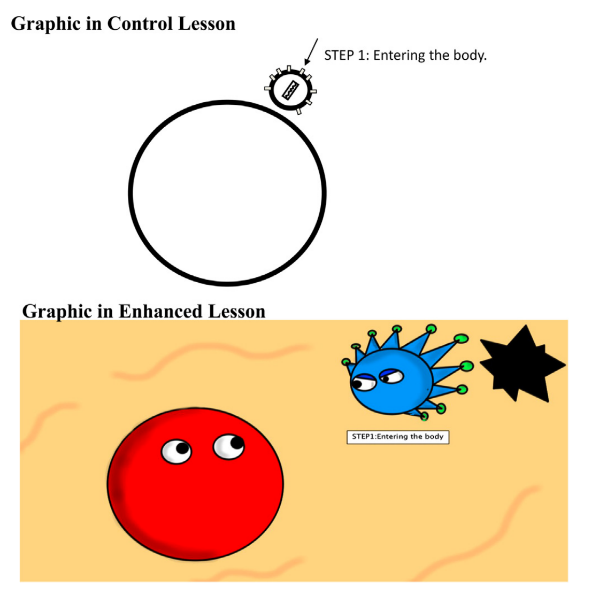
\includegraphics[width=0.7\linewidth]{graphics/Benefits_of_emotional_design_in_multimedia_instruction}
	\caption{Graphics from control and enhanced group. From \cite{Mayer2014}}
	\label{fig:benefits-bio-lesson}
\end{figure}	

% tables
\newpage
\section{Tables}
%\section{\\Table: Remote Associates Test}

\begin{table}[h!]
%	\centering
	\begin{tabular}{llll}
		\hline
		Remote Associate Item    & Solution & \pbox{20cm}{\% of participants \\ solving item (30 sec threshold)} & Used In \rule[-2ex]{0pt}{7ex} \\ [2ex] \hline
		political/surprise/line  & party    & 90\%                                               & main  		\\ [0.5ex]
		measure/worm/video       & tape     & 87\%                                               & main  		\\ [0.5ex]
		rocking/wheel/high       & chair    & 87\%                                               & main  		\\ [0.5ex]
		cracker/fly/fighter      & fire     & 85\%                                               & main  		\\ [0.5ex]
		nuclear/feud/album       & family   & 85\%                                               & main  		\\ [0.5ex]
		preserve/ranger/tropical & forest   & 85\%                                               & main  		\\ [0.5ex]
		water/mine/shaker        & salt     & 85\%                                               & main  		\\ [0.5ex]
		food/forward/break       & fast     & 82\%                                               & main  		\\ [0.5ex]
		sleeping/bean/trash      & bag      & 82\%                                               & main  		\\ [0.5ex]
		show/life/row            & boat     & 79\%                                               & main  		\\ [0.5ex]
		fish/mine/rush           & gold     & 74\%                                               & main  		\\ [0.5ex]
		high/district/house      & school   & 74\%                                               & main  		\\ [0.5ex]
		basket/eight/snow        & ball     & 72\%                                               & main  		\\ [0.5ex]
		opera/hand/dish          & soap     & 62\%                                               & main    		\\ [0.5ex]
		night/wrist/stop         & watch    & 97\%                                               & main    		\\ [0.5ex]
		dew/comb/bee             & honey    & 100\%                                              & main    		\\ [0.5ex]
		aid/rubber/wagon         & band     & 69\%                                               & main    		\\ [0.5ex]
		cane/daddy/plum          & sugar    & 97\%                                               & main    		\\ [0.5ex]
		fox/man/peep             & hole     & 64\%                                               & main    		\\ [0.5ex]
		loser/throat/spot        & sore     & 82\%                                               & main    		\\ [0.5ex]
		cream/skate/water        & ice      & 90\%                                               & practice     \\ [0.5ex]
		dust/cereal/fish         & bowl     & 49\%                                               & practice     \\ [0.5ex]
		cottage/swiss/cake       & cheese   & 94\%                                               & practice     \\ \hline
	\end{tabular}
	\caption{Selected items from Remote Associates Test \cite{Bowden}}
	\label{table:1}
\end{table}

% excerpts
\newpage
\section{Listings}


\begin{listing}[ht!]
\begin{itemize}
	\item You have advanced proficiency in English language
	\item You are not under time pressure
	\item You are not going through an abnormally stressful situation in
	your life
	\item You will be presented with photos that might be disturbing in
	nature, you are not dangerously susceptible to emotional stimuli.
	\item If you feel uncomfortable at any time you may stop the test, your
	participation will not be counted in this case
\end{itemize}

\label{itm:participation_requirements}
\caption{Excerpt: Participation requirements}
\end{listing}


\begin{listing}[ht!]
	\begin{minted}{sql}
	select users.index, 
	count(*)
	from df_live_sessions as sessions
	left join df_live_users as users on "userID"=users.index 
	where started is not null
	and finished is not null
	group by 1;
	\end{minted}
	
	\label{itm:sql_check_single_session_per_user}
	\caption{SQL Statement: Checks whether one user only has one session}
\end{listing}

\clearpage


% ---------------------------------------------------
% --- frontmatter: List of Excerpts ---
% ---------------------------------------------------
\renewcommand\listoflistingscaption{List of Excerpts}
\listoflistings
% ---------------------------------------------------
% --- frontmatter: List of Figures ---
% ---------------------------------------------------
\listoffigures
% ---------------------------------------------------
% --- frontmatter: List of Tables ---
% ---------------------------------------------------
\listoftables

\clearpage


\nocite{*}

\bibliographystyle{apalike}
\bibliography{../Library/Masterarbeit}

% Erzeugen der Selbständigkeitserklärung auf einem neuen Blatt:
\selbstaendigkeitserklaerung{\today}

%%{\Large{\bf Declaration of Authorship}}\vspace{0.5cm}

\section*{Declaration of Authorship}

I hereby confirm that I have authored this Master's
thesis independently and without use of others than the indicated
sources. All passages which are literally or in general matter
taken out of publications or other sources are marked as such.
\vspace{1cm}

Berlin, \today \vspace{0.5cm}

Oleg Bystrov


\end{document}